
\section{Singlecross Calculus (SCC)}\label{sec:single-cross}

\kasten{
\subsubsection*{Singlecross calculus (SCC) overview}
\begin{calcfeatures}
\feature{calculus identifier}{scc}
\feature{calculus parameters}{none}
\feature{arity}{ternary}
\feature{entity type}{2D points}
\feature{description}{relates the referent c relative to the line between origin a and relatum b and the orthogonal line thru b, resulting in 11 base relations}
\feature{base relations}{0..7 and b (for b=c), dou, tri}
\lastfeature{references}{\citet{cosyfre92}}
\end{calcfeatures}
}

The single cross calculus is a ternary calculus that describes the direction of
a point $C$ (the referent) with respect to a point $B$ (the relatum) as seen
from a third point $A$ (the origin). It has originally been proposed in
\citet{cosyfre92}. The plane is partitioned into regions by the line going
through $A$ and $B$ and the perpendicular at $B$. This results in eight
possible directions for $C$ as illustrated in Fig.~\ref{fig:SCC}. We denote
these base relations by numbers from 0 to 7 instead of using linguistic
prepositions, e.g. 2 instead of \emph{left}, as originally done in
\citet{cosyfre92}. Relations 0, 2, 4, 6 are linear ones, while relations 1, 3,
5, 7 are planar. In addition, three special relations exist for the cases $A\neq
B=C$ (\textbf{b}), $A=B \neq C$ (\textbf{dou}), and $A=B=C$ (\textbf{tri}). A
single cross relation $rel_{SCC}$ is written as $A,B \; rel_{SCC}\; C$,
e.g. $A,B\; \textbf{4}\; C$ or $A,B\,\, \textbf{dou}\; C$. The relation depicted in Fig.~\ref{fig:SCC} is the relation $A,B\; \textbf{5}\; C$.

\begin{figure}[ht]
	\centering
	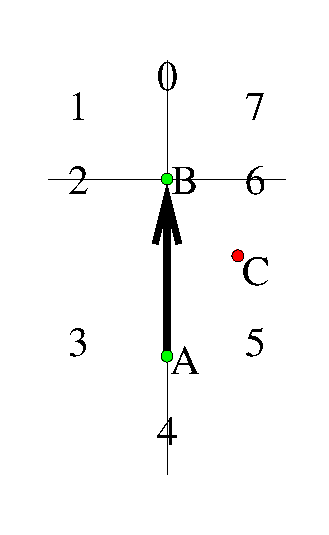
\includegraphics[height=4.3cm]{Singlecross}
	\caption{The Single Cross Reference System}
	\label{fig:SCC}
\end{figure}
